\documentclass[11pt,twocolumn]{article}
\setlength{\columnsep}{0.5cm}

\usepackage[utf8]{inputenc}
\usepackage[T1]{fontenc}
\usepackage[spanish]{babel}
\usepackage{hyperref}
\usepackage{graphicx}

\title{\vspace{-15mm}%
	\fontsize{24pt}{10pt}\selectfont
	\textbf{WikiPapers: a collaborative compilation of wiki research literature... in a wiki!}
	}	
\author{%
	\large
	\textsc{Emilio J. Rodríguez-Posada} \\
	\normalsize	Private \\
	\normalsize	\href{mailto:emijrp@gmail.com}{emijrp@gmail.com}
	\vspace{-5mm}
	}
\date{}


\begin{document}


\twocolumn[
  \begin{@twocolumnfalse}

    \maketitle

\begin{abstract}
  El interés de los investigadores por los wikis, en especial Wikipedia, ha ido creciendo en los últimos años. La primera edición de WikiSym, un simposio sobre wikis, se celebró en 2005 y desde entonces han aparecido congresos, workshops, conferencias y competiciones. El estudio de los wikis es un campo emergente y prolífico. Por ello, ha habido varios intentos de recopilar toda la literatura sobre wikis, aunque con escaso éxito. Unas veces el enfoque o la herramienta utilizada eran limitados, otras veces el proyecto era abandonado y al poco tiempo los metadatos bibliográficos se perdían. En este artículo presentamos WikiPapers, un proyecto colaborativo para recopilar toda la literatura sobre wikis. Se hace uso de MediaWiki y su extensión semántica, ambos conocidos por los investigadores de este área. Hasta octubre de 2012 se han recopilado más de 1.400 publicaciones y sus metadatos, además de documentación sobre herramientas y datasets relacionados. Los metadatos son exportables en los formatos BibTeX, RDF, CSV y JSON. Los dumps del wiki con sus historiales están disponibles para descarga.
\end{abstract}

  \end{@twocolumnfalse}
  ]
	

\section{Introducción}
El interés de los investigadores por los wikis, en especial Wikipedia, ha ido creciendo en los últimos años. La primera edición de WikiSym, un simposio sobre wikis, se celebró en 2005 y desde entonces han aparecido congresos como CLEF/PAN Lab, workshops como WikiAI, SemWiki y MathWikis, conferencias como Wikimania, WikiCon, SMWCon, Wiki Conference India, Wikipedia Academy y Wikipedia CPOV Conference y competiciones como WikiViz. El estudio de los wikis es un campo emergente y prolífico.

\section{Trabajos relacionados}
Ha habido varios intentos de recopilar toda la literatura científica sobre wikis, aunque con poco éxito. Unas veces el enfoque o la herramienta utilizada eran limitados, otras veces el proyecto era abandonado y al poco tiempo los metadatos bibliográficos se perdían. Se han hecho recopilaciones en páginas personajes y blogs, a través de revisiones de literatura, haciendo uso de gestores de bibliografía, en páginas de Wikipedia y también en servicios como Zotero o CiteULike. Todos tienen inconvenientes.

\subsection{Páginas personales y blogs}
Existen ejemplos de recopilaciones de literatura en webs personales\footnote{\href{http://www.public.iastate.edu/~CYBERSTACKS/WikiBib.htm}{http://www.public.iastate.edu/~CYBERSTACKS/WikiBib.htm}} y blogs. Un ejemplo bastante completo de este último es SWEETpedia,\footnote{\href{http://www.mkbergman.com/sweetpedia/}{http://www.mkbergman.com/sweetpedia/}} que contiene publicaciones sobre wikis y semántica. Uno de los inconvenientes de este sistema es que el esfuerzo suele recaer sobre una única persona y los metadatos no son fácilmente exportables.

\subsection{Revisiones de literatura}
Se han realizado varias revisiones de literatura hasta el momento. La primera de ellas (Voss, 2005) se hizo en un momento en el que las publicaciones eran escasas, pero ya se intuía que estaba en crecimiento. Un año más tarde (Ayers, 2006) vuelve a hacer un repaso a la literatura existente.

No sería hasta 3 años después cuando (Okoli et al., 2009) presentan una propuesta de protocolo para hacer un mapeo sistemático y ese mismo año (Okoli, 2009) analiza el estdo del arte.

(Nielsen, 2011) hace la mayor revisión de literatura en un documento de más de 50 páginas, en progreso e inacabado, que incluye 300 referencias a publicaciones y asegura haber encontrado más de 1.000 publicaciones sobre el tema.

(Martin, 2011)

(Okoli, 2012)

(Jullien, 2012)

Uno de los inconvenientes de estas revisiones de literatura es que quedan rápidamente desactualizadas debido al ritmo con el que aparecen nuevas publicaciones.

\subsection{Gestores bibliográficos}
Se han empleado gestores bibliográficos específicos como WIKINDX\footnote{\href{http://sourceforge.net/projects/wikindx/}{http://sourceforge.net/projects/wikindx/}} creando portales como Wikibibliographie ENCYCLEN\footnote{\href{http://wikindx.inrp.fr/biblio_encyclen/}{http://wikindx.inrp.fr/biblio\_encyclen/}} pero restringen la edición a un círculo de usuarios aprobados.

%\href{http://toolserver.org/~voj/bibliography/}{http://toolserver.org/~voj/bibliography/}
%\href{http://wikiindex.org/Wiki_Research_Bibliography}{http://wikiindex.org/Wiki\_Research\_Bibliography}

\subsection{Páginas individuales en Wikipedia}
También existen listados de publicaciones y recursos en algunas Wikipedias, como en la versión alemana\footnote{\href{http://de.wikipedia.org/wiki/Wikipedia:Wikipedistik/Bibliographie}{http://de.wikipedia.org/wiki/Wikipedia:Wikipedistik/Bibliographie}} y la inglesa\footnote{\href{http://en.wikipedia.org/wiki/Wikipedia:Academic_studies_of_Wikipedia}{http://en.wikipedia.org/wiki/Wikipedia:Academic\_studies\_of\_Wikipedia}}. El principal inconveniente es que no es posible jugar con los datos dentro del mismo wiki, al estar todo escrito como texto plano, sin enriquecimiento semántico.

\subsection{Servicios web y redes sociales}
Finalmente servicios web y redes sociales con recopilaciones de literatura sobre wikis. Es el caso de grupos de Zotero,\footnote{\href{https://www.zotero.org/groups/wikipedia_research}{https://www.zotero.org/groups/wikipedia\_research}} tags de BibSonomy\footnote{\href{http://www.bibsonomy.org/tag/wikipedia}{http://www.bibsonomy.org/tag/wikipedia} y \href{http://www.bibsonomy.org/tag/wiki}{http://www.bibsonomy.org/tag/wiki}} y grupos y tags de CiteULike.\footnote{\href{http://www.citeulike.org/tag/wikipedia}{http://www.citeulike.org/tag/wikipedia}, \href{http://www.citeulike.org/tag/wiki}{http://www.citeulike.org/tag/wiki} y \href{http://www.citeulike.org/group/382}{http://www.citeulike.org/group/382}}

\section{WikiPapers}
WikiPapers\footnote{\href{http://wikipapers.referata.com}{http://wikipapers.referata.com}} fue lanzado en abril de 2011. Haciendo uso de MediaWiki y su extensión semántica, recopila de manera colaborativa información acerca de toda la literatura científica sobre wikis, así como de herramientas y datasets relacionados. No hace falta estar registrado para participar, pero es recomendable.

WikiPapers agrupa todas las ventajas de los sistemas mencionados anteriormente y soluciona sus inconvenientes. Permite hacer listados de publicaciones similares a SWEETpedia: existe uno de revisiones de literatura por poner solo un ejemplo.\footnote{\href{http://wikipapers.referata.com/wiki/List_of_literature_reviews}{http://wikipapers.referata.com/wiki/List\_of\_literature\_reviews}} Funciona como un gestor bibliográfico, al almacenar los metadatos de las publicaciones y permitir hacer búsquedas, filtrarlos o exportarlos, individualmente o en conjunto. También facilita que grupos de usuarios se comuniquen a través de las páginas de discusión y compartan información sobre publicaciones de su interés, funcionando como una red social. El espacio de discusión debajo de cada página posibilita a los lectores hacer valoraciones de los artículos.

Desde un punto de vista más estadístico, es posible generar gráficas a partir de los metadatos disponibles en WikiPapers, aprovechando así la capacidad que ofrece la semántica. Gráficos de barras, circulares o líneas temporales están presentes y facilitan la visualización y comprensión de la información.

Finalmente, el wiki y sus historiales están disponibles tanto para su descarga como dump XML y accesible a través de la API de MediaWiki. Esto impide que todo el trabajo se pierda, como sucedió en algún proyecto del pasado.

\begin{figure}[htb]
\centering
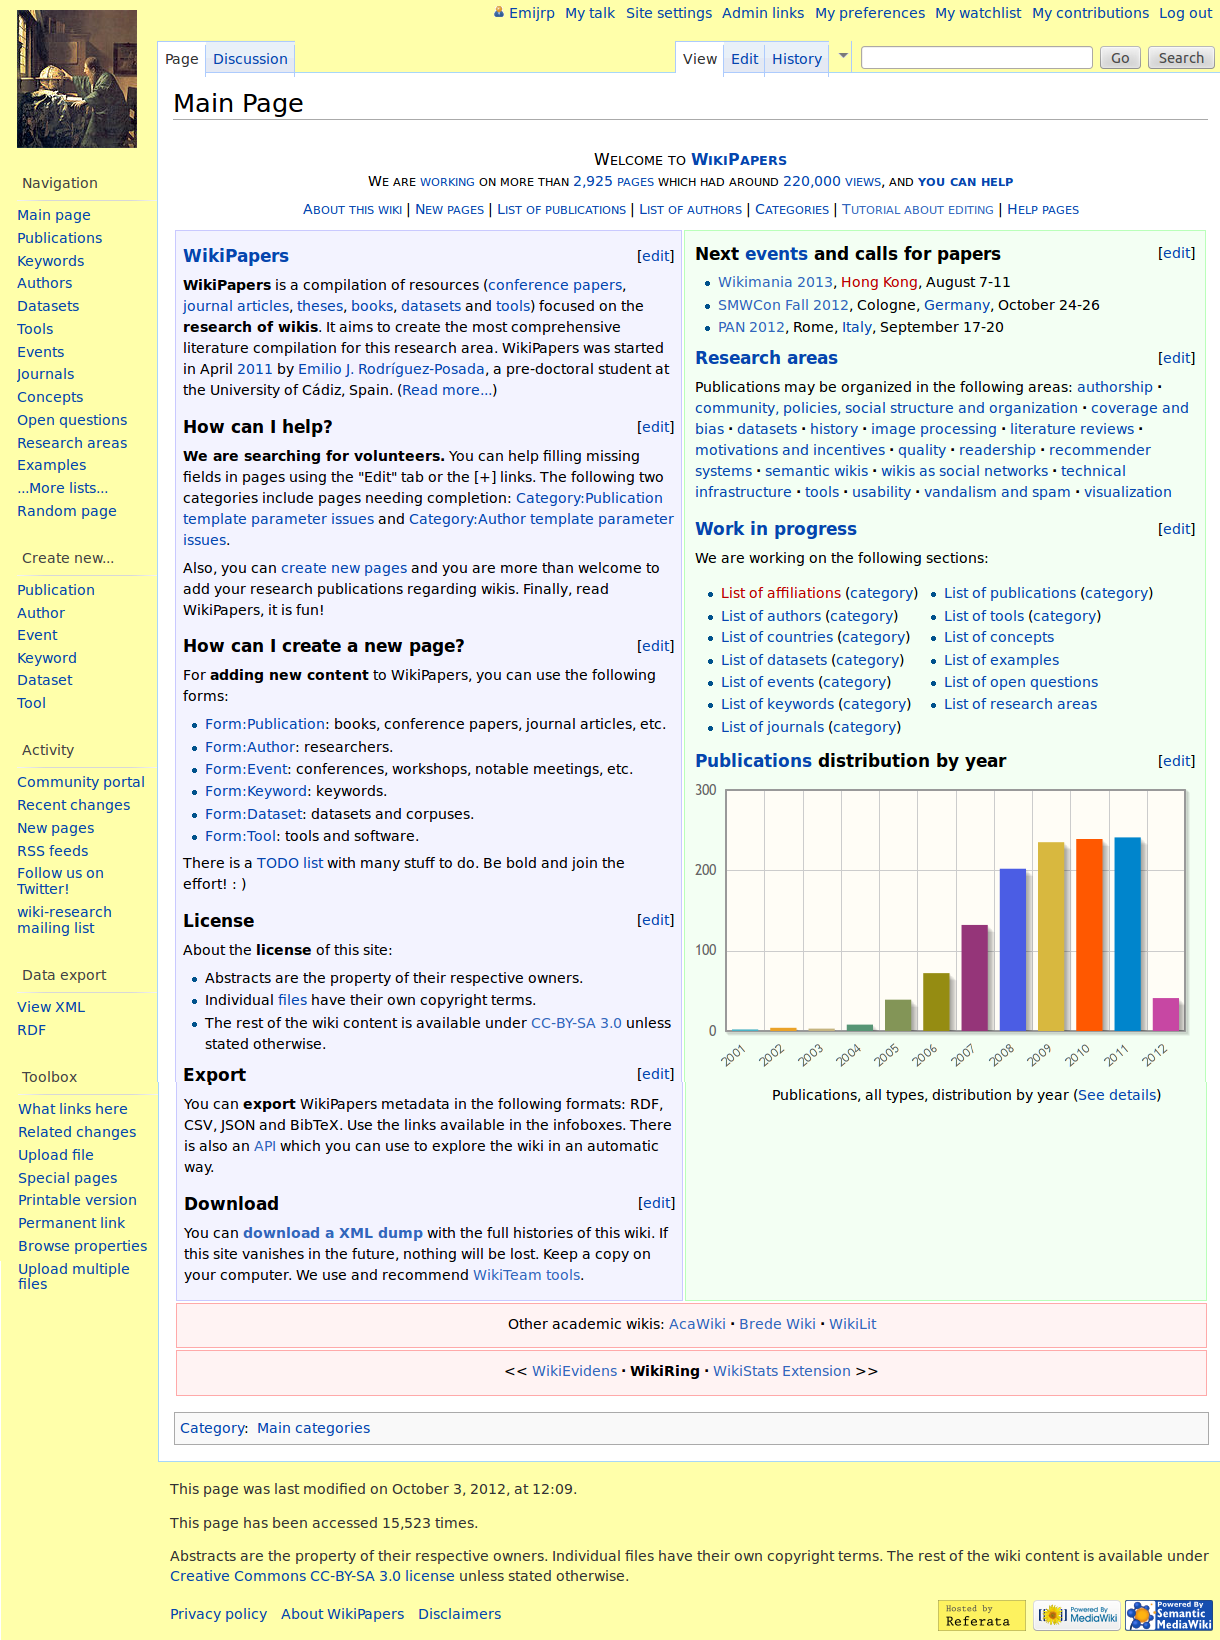
\includegraphics[width=0.49\textwidth]{wpfull.png}
\caption{Portada de WikiPapers}
\label{fig:wpfull}
\end{figure}

\subsection{Publicaciones}
En WikiPapers cada publicación dispone de una página en la que se detallan todos sus metadatos (título, autores, palabras clave, año, revista o congreso, DOI, idioma, licencia, enlaces al fichero y motores de búsqueda), el abstract, las referencias que incluye y las citas que recibe, y un espacio de discusión. Los metadatos sirven para hacer búsquedas y filtrar los contenidos. A octubre de 2012 ya cuenta con más de 1.400 publicaciones, incluyendo artículos de revistas y congresos, tesis y libros.

\subsection{Autores}
Para cada autor existe una ficha que incluye su nombre, afiliación, país, índice de coautores, página web, y por supuesto un listado de publicaciones, datasets y herramientas de las que es autor.

\subsection{Herramientas}
Repaso a las herramientas

\subsection{Datasets}
Repaso a los datasets, los wikis como datasets (WIkiTeam)

\subsection{Eventos}
ya están nombrados en el abstract y la intro...

\subsection{Y más...}
También hay información sobre conceptos, ejemplos, preguntas abiertas, encuestas, motores wiki, wikifarms.
Los autores pueden presentarse un poco en sus páginas de usuario.
Posibilidad de incrustar diapositivas (por ejemplo SlideShare) y vídeos (YouTube, Vimeo...).

\subsection{Reutilización}
Posibilidades de reutilizar el contenido ….
Todos los metadatos se pueden exportar en los formatos BibTeX, RDF, CSV y JSON.
Comentar que WikiLit ha cogido las plantillas y estructura de WikiPapers para crear su propio review de la literatura, limitado a revistas... ?

\section{Conclusiones y trabajo futuro}
porqué hacía falta WikiPapers
aglutina todas las ventajas de los anteriores sistemas
lo que se ha hecho, cifras,
lo que queda por hacer y como ayudar
el futuro y más allá...

\section{Agradecimientos}
...

\section{Referencias}
Voss, J. (2005). Measuring Wikipedia. In the International Conference of the International Society for Scientometrics and Informetrics.

Ayers, P. (2006). Researching Wikipedia -- Current approaches and new directions. Proceedings of the American Society for Information Science and Technology

Okoli, C. and Schabram, K. (2009). Protocol for a systematic literature review of research on the Wikipedia. International Conference on Management of Emergent Digital EcoSystems

Okoli, C. (2009). A Brief Review of Studies of Wikipedia in Peer-Reviewed Journals. Third International Conference on Digital Society
Nielsen, F. A. (2011). Wikipedia research and tools: Review and comments.

Martin, O. S. (2011). A Wikipedia Literature Review.
Okoli, C., Mehdi, M., Mesgari, M., Nielsen, F. A.,  Lanam\"{a}ki, A. (2012). The people's encyclopedia under the gaze of the sages: a systematic review of scholarly research on Wikipedia.

Jullien, N. (2012). What We Know About Wikipedia: A Review of the Literature Analyzing the Project(s).

\section{Licencia}
Este obra está bajo licencia \href{http://creativecommons.org/licenses/by-sa/3.0/}{Creative Commons Reconocimiento-CompartirIgual 3.0 Unported}.

\end{document}
